\section{Udregn anbefalet hastighed}
\begin{frame}{Modellen}
\begin{itemize}
\item Biler (id, position, acceleration og deceleration)
\item Faser (fx. $\langle(green, 30), (yellow, 4), (red, 30), (yellow, 2)\rangle$)
\item Kort (orienteret graf med kanter, knuder og forbindelser)
\item Kryds (samling af forbindelser)
\item Ruter (sekvens af kanter forbundet med forbindelser)
\end{itemize}

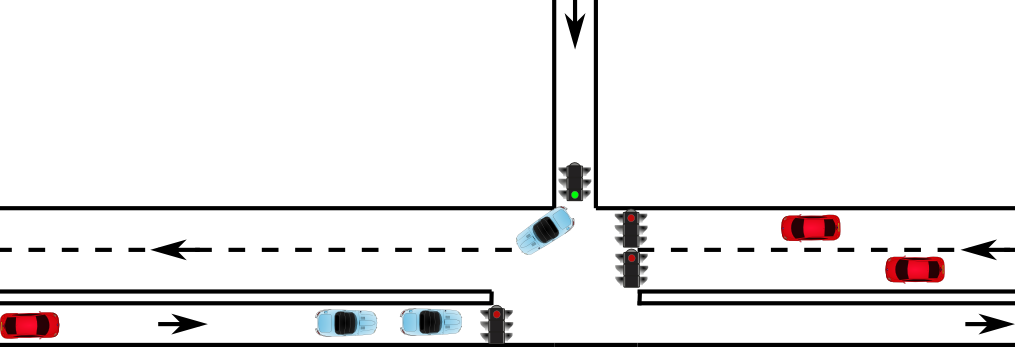
\includegraphics[width=1\textwidth]{../images/introNetworkSimple.png}
\end{frame}

\begin{frame}{Kort}
Bruger SUMO's model
\begin{itemize}
\item Orienteret kanter mellem to knuder
	\begin{itemize}
	\item Tilknyttet fartgrænse og antal baner
\end{itemize}
\item Orienteret forbindelser: 
	\begin{itemize}
	\item Art kanter med tilknyttet fase
	\item Angiver tilladte forbindelser mellem kanters baner
	\end{itemize}
\end{itemize}

\vspace{5mm}
\begin{center}
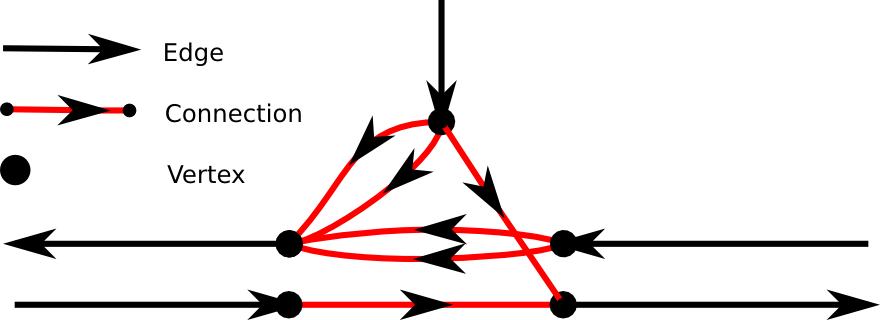
\includegraphics[width=0.8\textwidth]{../images/ConnectionNetwork.png}
\end{center}
\end{frame}

\begin{frame}{Modellen}
\begin{itemize}
\item Biler (id, position, acceleration og deceleration)
\item Faser (fx. $\langle(green, 30), (yellow, 4), (red, 30), (yellow, 2)\rangle$)
\item Kort (orienteret graf med kanter, knuder og forbindelser)
\item Kryds (samling af forbindelser)
\item Ruter (sekvens af kanter forbundet med forbindelser)
\end{itemize}

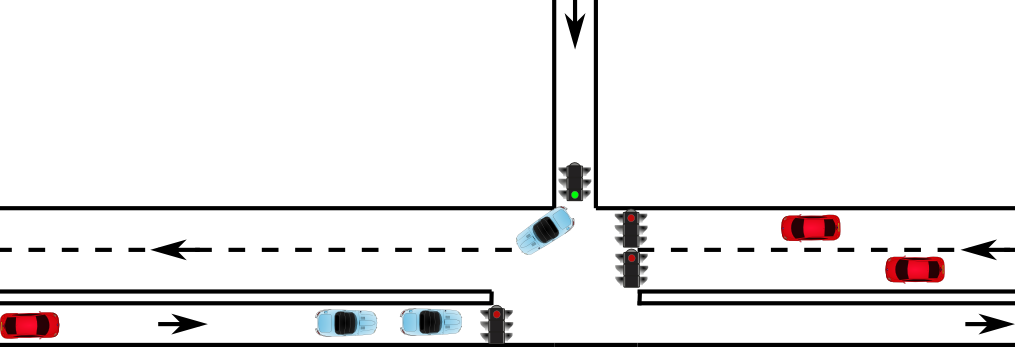
\includegraphics[width=1\textwidth]{../images/introNetworkSimple.png}
\end{frame}